\documentclass[11pt]{article}

\IfFileExists{lmodern.sty}{\usepackage[T1]{fontenc}\usepackage{lmodern}}{\usepackage[T1,OT1]{fontenc}\PassOptionsToPackage{expansion=false}{microtype}}
\newcommand{\eogonek}{{\fontencoding{T1}\selectfont\k{e}}}% the letter e with ogonek, for Naskr\eogonek cki
\usepackage[margin=1.1in]{geometry}
\usepackage{amsmath,amssymb,amsthm}
\usepackage{microtype}
\usepackage{booktabs}
\usepackage{tabularx}
\usepackage{enumitem}
\usepackage{xcolor}
\usepackage{tikz}
\usetikzlibrary{arrows.meta,positioning,decorations.pathreplacing,calc}
\usepackage[most]{tcolorbox}
\usepackage[colorlinks=true,linkcolor=blue!50!black,citecolor=blue!50!black,urlcolor=blue!50!black]{hyperref}
\usepackage[capitalise,nameinlink,noabbrev]{cleveref}

% ------------------------------------------------------------------
% Environments for the note itself
% ------------------------------------------------------------------
\theoremstyle{plain}
\newtheorem{theorem}{Theorem}[section]
\newtheorem{proposition}[theorem]{Proposition}
\newtheorem{corollary}[theorem]{Corollary}
\theoremstyle{definition}
\newtheorem{definition}[theorem]{Definition}
\newtheorem{procedure}[theorem]{Procedure}
\theoremstyle{remark}
\newtheorem{remark}[theorem]{Remark}

\crefname{procedure}{Procedure}{Procedures}

% ------------------------------------------------------------------
% Environments for the worked HFF example (Section 7)
% ------------------------------------------------------------------
\newcounter{hffc}
\theoremstyle{definition}
\newtheorem{hffdef}[hffc]{Definition}
\theoremstyle{plain}
\newtheorem{hfflem}[hffc]{Lemma}
\newtheorem{hffthm}[hffc]{Theorem}
\theoremstyle{remark}
\newtheorem{hffrem}[hffc]{Remark}
\crefname{hffdef}{Definition}{Definitions}
\crefname{hfflem}{Lemma}{Lemmas}
\crefname{hffthm}{Theorem}{Theorems}
\crefname{hffrem}{Remark}{Remarks}

% The separator mark of an HFF document
\newcommand{\HFFmark}{\par\medskip\begin{center}{\Large$\maltese$}\end{center}\medskip\par}

% Length annotation, shown next to the QED symbol in the worked example
\newcommand{\hffcost}{}
\newcommand{\setcost}[1]{\renewcommand{\hffcost}{#1}}

\renewcommand{\labelitemi}{$\bullet$}% vector bullet even without cm-super
\newcommand{\HFF}{\textsc{hff}}

\title{Checking AI-Generated Proofs:\\[0.3em] \large The Human Friendly Form}
\author{Siddharth Iyer}
\date{October 2026}

\begin{document}

\maketitle

\begin{abstract}
Suppose an AI system has produced a proof of a theorem $T$. This note proposes a way for a human to convince themselves that the proof is correct by reading it, without relying on a proof assistant. The AI is asked to write the proof in a prescribed format, the \emph{Human Friendly Form} (\HFF): a plain-English overview, then, after a distinguished mark, a proof written entirely as definitions, lemmas and remarks, in which every lemma is proved directly below its statement in fewer than a fixed number of visible characters, and finally a list of references. Alongside the document, the AI produces a \emph{map}: an interactive two-dimensional rendering of the dependency graph of the definitions and lemmas, which the reader explores as one explores the map of a strategy game. Checking the proof then reduces to checking a list of short, independent steps in any order, and the map records which steps have been checked.
\end{abstract}

% ==================================================================
\section{Introduction}
% ==================================================================

Suppose that an AI system has produced a proof of a theorem $T$. When is a human entitled to be happy with it? In this note we take the answer to be: when they have convinced themselves that the proof is correct, by checking it as a careful referee checks a paper. We do not assume that the proof has been formalised in a proof assistant, and we set aside the harder question of what it would mean to understand the proof, as well as the broader question, taken up by Tao~\cite{Tao}, of what the goals and values of mathematical research become once AI tools can do research-level mathematics. The question of correctness is a pressing one. The recent Leiden Declaration on Artificial Intelligence and Mathematics~\cite{Leiden} warns that automated tools can produce arguments that look plausible but are unreliable or even wrong, and that are hard to tell apart from correct proofs; it also holds that responsibility for the correctness of a result stays with its human authors. The aim of this note is to make that responsibility practical to discharge by hand.

Checking an AI-generated proof in its raw form can be hard for reasons that have little to do with the mathematics. The argument may be long and unbroken, auxiliary claims may be proved inline and used much later, routine and delicate steps may be interleaved without signposting, and the dependencies between the parts may be left implicit. The referee then has to hold large parts of the argument in mind at once, and an error can hide in the middle of a long paragraph.

On the other hand, rewriting a proof into a different shape costs the AI almost nothing, while the reader's attention is scarce. We therefore ask the AI to write its proof in a form designed for checking, the \emph{Human Friendly Form} (\HFF). It has three ingredients:
\begin{itemize}[leftmargin=2em]
  \item an \textbf{overview} in plain English, so that the reader knows what is proved and by what strategy before checking any detail;
  \item a \textbf{map} of the dependency graph of the proof, through which the reader navigates and on which they record their progress;
  \item a proof written entirely in \textbf{small blocks}, with every lemma proved in fewer than $L$ visible characters, so that each block can be checked in a single sitting.
\end{itemize}
The last ingredient rests on a simple local-to-global principle (\cref{prop:local-global}): if every block has been checked, taking the statements it cites as given, then $T$ has been proved. Checking the proof becomes a list of small, independent tasks.\footnote{Throughout, $T$ denotes the main theorem and $L$ the length budget for proofs, counted in visible characters of the compiled document (\cref{sec:formulas}). A reasonable default is $L = 300$, about four or five typeset lines.}

% ==================================================================
\section{The Human Friendly Form}\label{sec:hff}
% ==================================================================

\begin{definition}[Blocks]\label{def:block}
A \emph{block} is one of the following.
\begin{enumerate}[label=(\alph*)]
  \item A \emph{definition}: a header and a body introducing a notion or a piece of notation.
  \item A \emph{lemma}: a header, a statement, and a proof placed immediately below the statement. The main theorem $T$ is a distinguished lemma, typeset as ``Theorem''.
  \item A \emph{remark}: a header and free text.
\end{enumerate}
Blocks are numbered consecutively in a single sequence, whatever their kind, so that each number names exactly one block: a document might begin with Definition~1, Lemma~2, Remark~3. The \emph{header} of a block is its number together with a short descriptive name, for instance ``Lemma 5 (Prime factor $\equiv 3 \bmod 4$)''.
\end{definition}

\begin{definition}[Citations and the dependency graph]\label{def:graph}
A block $v$ \emph{cites} a definition or lemma $u$ if the statement or the proof of $v$ uses $u$; citations must be explicit, by number. The \emph{dependency graph} $G$ of a document is the directed graph whose vertices are its definitions and lemmas, with an edge $u \to v$ whenever $v$ cites $u$. Remarks are not vertices of $G$.
\end{definition}

\begin{definition}[Human Friendly Form]\label{def:hff}
A document is in \emph{Human Friendly Form} for $T$, with budget $L$, if it satisfies the following conditions.
\begin{enumerate}[label=\textbf{(H\arabic*)}, leftmargin=3.2em]
  \item\label{H:overview} \textbf{Overview.} It opens with \emph{Part~I}, at most a few pages of English prose, which states $T$ in words and describes the methods used to prove it: the overall strategy, the techniques involved, and which steps are routine and which are delicate.
  \item\label{H:mark} \textbf{Separator.} Part~I is followed by a line containing only the mark $\maltese$. Everything after the mark, up to the references, is \emph{Part~II}, the proof.
  \item\label{H:graph} \textbf{The map.} The document is accompanied by a separate file, the \emph{map}, which renders $G$ interactively (\cref{sec:map}). A static drawing of $G$ may also be placed directly after the mark, but it is optional.
  \item\label{H:blocks} \textbf{Block discipline.} In Part~II, every piece of text belongs to a definition, a lemma or a remark. There is no free-standing prose; the only other thing allowed is the optional drawing of $G$.
  \item\label{H:short} \textbf{Short proofs.} The proof of each lemma appears directly below its statement and has length less than $L$, where length is the number of visible characters in the compiled document (\cref{sec:formulas}).
  \item\label{H:order} \textbf{Well-founded order.} Each block cites only blocks that appear before it. In particular $G$ is acyclic, and the order of the document is a topological order of $G$.
  \item\label{H:sink} \textbf{Single goal.} $T$ is the last lemma, and every vertex of $G$ has a directed path to $T$.
  \item\label{H:inert} \textbf{Inert remarks.} Remarks carry no logical weight: deleting every remark leaves a complete proof of $T$. In particular, no block cites a remark.
  \item\label{H:refs} \textbf{References.} The document ends with a list of references, as any paper does, whenever it draws on the literature. Part~I and the remarks may cite it freely, and every imported lemma (\cref{rem:imported}) must.
\end{enumerate}
\end{definition}

\Cref{fig:anatomy} shows the shape of such a document.

\begin{figure}[ht]
\centering
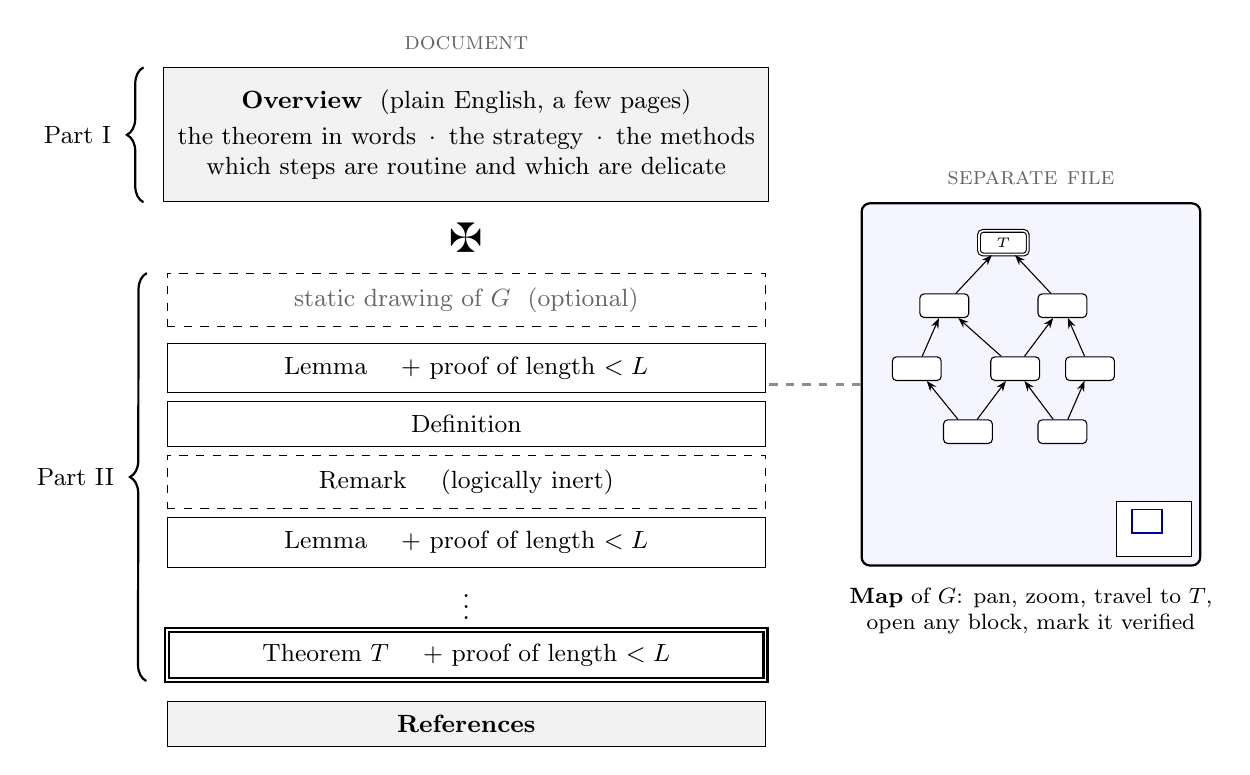
\begin{tikzpicture}[
  blk/.style={draw, minimum width=7.6cm, align=center, font=\small, inner sep=5pt},
  brace/.style={decorate, decoration={brace, amplitude=6pt, mirror}, thick},
  mv/.style={draw, rounded corners=1.5pt, minimum width=0.62cm, minimum height=0.3cm, inner sep=0pt, fill=white, font=\tiny},
  me/.style={-{Stealth[length=1.3mm]}, thin}
]
% --- the document ---
\node[font=\small\scshape, text=black!60] (doclabel) {document};
\node[blk, below=1mm of doclabel, minimum height=1.7cm, fill=black!5] (p1) {\textbf{Overview} \ (plain English, a few pages)\\[2pt]
  the theorem in words \,$\cdot$\, the strategy \,$\cdot$\, the methods\\
  which steps are routine and which are delicate};
\node[below=1.5mm of p1, font=\Large] (mark) {$\maltese$};
\node[blk, below=1.5mm of mark, dashed, text=black!60] (g) {static drawing of $G$ \ (optional)};
\node[blk, below=2mm of g] (b1) {Lemma \quad + proof of length $< L$};
\node[blk, below=1mm of b1] (b2) {Definition};
\node[blk, below=1mm of b2, dashed] (b3) {Remark \quad (logically inert)};
\node[blk, below=1mm of b3] (b4) {Lemma \quad + proof of length $< L$};
\node[below=0mm of b4] (dots) {$\vdots$};
\node[blk, below=0mm of dots, double, thick] (bn) {Theorem $T$ \quad + proof of length $< L$};
\node[blk, below=2.5mm of bn, fill=black!5] (refs) {\textbf{References}};
\draw[brace] ($(p1.north west)+(-0.25,0)$) -- node[left=8pt, font=\small] {Part I} ($(p1.south west)+(-0.25,0)$);
\draw[brace] ($(g.north west)+(-0.25,0)$) -- node[left=8pt, font=\small] {Part II} ($(bn.south west)+(-0.25,0)$);
% --- the map ---
\node[draw, thick, rounded corners=3pt, fill=blue!4, minimum width=4.3cm, minimum height=4.6cm, anchor=north west] (map) at ($(g.north east)+(1.2,0.9)$) {};
\node[font=\small\scshape, text=black!60, above=1mm of map] {separate file};
\begin{scope}[shift={($(map.center)+(-0.35,0.25)$)}]
  \node[mv, double] (mT) at (0,1.55) {$T$};
  \node[mv] (m1) at (-0.75,0.75) {};
  \node[mv] (m2) at (0.75,0.75) {};
  \node[mv] (m3) at (-1.1,-0.05) {};
  \node[mv] (m4) at (0.15,-0.05) {};
  \node[mv] (m5) at (1.1,-0.05) {};
  \node[mv] (m6) at (-0.45,-0.85) {};
  \node[mv] (m7) at (0.75,-0.85) {};
  \draw[me] (m1) -- (mT); \draw[me] (m2) -- (mT);
  \draw[me] (m3) -- (m1); \draw[me] (m4) -- (m1); \draw[me] (m4) -- (m2); \draw[me] (m5) -- (m2);
  \draw[me] (m6) -- (m3); \draw[me] (m6) -- (m4); \draw[me] (m7) -- (m4); \draw[me] (m7) -- (m5);
\end{scope}
\node[draw, fill=white, minimum width=0.95cm, minimum height=0.7cm, anchor=south east, inner sep=0pt] (mini) at ($(map.south east)+(-0.12,0.12)$) {};
\draw[blue!60!black, semithick] ($(mini.center)+(-0.28,-0.05)$) rectangle ($(mini.center)+(0.1,0.25)$);
\node[below=1.5mm of map, font=\footnotesize, align=center] (maptext) {\textbf{Map} of $G$: pan, zoom, travel to $T$,\\ open any block, mark it verified};
\draw[dashed, black!45, thick] (map.west) -- (map.west -| b1.east);
\end{tikzpicture}
\caption{The anatomy of an \HFF{} document and its map. In Part~II, definitions, lemmas and remarks may appear in any order in which each block cites only earlier blocks \ref{H:order}; the order shown is one possibility, and the main theorem always comes last \ref{H:sink}.}\label{fig:anatomy}
\end{figure}

\begin{remark}[What the conditions are for]
Conditions \ref{H:blocks} and \ref{H:short} make every step small. Conditions \ref{H:order} and \ref{H:sink} make $G$ acyclic with $T$ as its only sink, which is exactly what is needed for checking every block to suffice (\cref{prop:local-global}); without \ref{H:order}, a cycle in $G$ would be a circular argument hiding in plain sight. Condition~\ref{H:inert} lets the reader skip every remark while checking, since remarks carry only motivation and heuristics. Condition~\ref{H:refs} is the convention of every paper, stated only because \ref{H:blocks} might otherwise seem to forbid a bibliography.
\end{remark}

\begin{remark}[Imported results]\label{rem:imported}
A proof of $T$ will usually rely on theorems from the literature, which cannot be reproved within the budget. We therefore allow an \emph{imported lemma}: a statement with a precise citation of the reference list, including the theorem number, in place of a proof. Imported lemmas are leaves of $G$ and are drawn distinctly on the map. They mark the trust boundary of the document, and the reader must check that each imported statement agrees \emph{exactly} with its source, hypotheses included; this is a common place for errors to hide.
\end{remark}

\begin{remark}[No hidden content in definitions]\label{rem:hidden}
Definitions have no proofs, which makes them a natural hiding place for unproved claims, as in ``let $f$ be the unique function such that\,\dots''. Any existence, uniqueness or well-definedness claim implicit in a definition must therefore be a separate lemma, which the definition cites and which, by \ref{H:order}, appears before it.
\end{remark}

\begin{remark}[The map is checked against the text]\label{rem:computed}
Since $G$ is determined by the citations, the map need not be taken on trust: its data can be generated from the source of the document by a script, or, if the AI writes it, compared with the source by a script. This is why \cref{def:graph} insists that citations be explicit: ``by the previous lemma'' should read ``by Lemma~4''.
\end{remark}

% ==================================================================
\section{The map}\label{sec:map}
% ==================================================================

A drawing of $G$ on a printed page works for a dozen vertices. The dependency graph of a serious proof may have hundreds, and is then better explored than looked at. The model is the map of a real-time strategy game such as \emph{Age of Empires}~\cite{AoE}: a large two-dimensional world of which the screen shows one window at a time, with a minimap in the corner showing the whole world and where the window currently is. The reader moves around with the mouse, the trackpad, a touch screen or the keyboard.

\begin{definition}[Map]\label{def:map}
A \emph{map} of an \HFF{} document is an interactive rendering of its dependency graph $G$ with the following features.
\begin{enumerate}[label=\textbf{(M\arabic*)}, leftmargin=3.2em]
  \item\label{M:layout} \textbf{Layout.} Each vertex $v$ is placed in a horizontal layer according to its \emph{depth}, the length of the longest directed path from $v$ to $T$, with $T$ alone at the top. Every edge points upward, so moving up the map means moving towards the theorem.
  \item\label{M:nav} \textbf{Navigation.} The reader pans by dragging and zooms with the scroll wheel or a pinch. A minimap shows the whole graph and the current window. A single key travels to $T$, and a search box travels to any block by number or by words in its header.
  \item\label{M:zoom} \textbf{Semantic zoom.} Zoomed out, each vertex shows only its number; at middle range, its header; zoomed in, its full statement.
  \item\label{M:open} \textbf{Opening a block.} Selecting a vertex opens its block beside the map: statement, proof, the length of the proof, and the blocks it uses and that use it, each a link that moves the window there. The paths from the vertex up to $T$ are highlighted.
  \item\label{M:status} \textbf{Verification status.} Each vertex is marked \emph{unverified} or \emph{verified} as the reader goes. Every unverified vertex lies under a dense fog, as unexplored land does in a strategy game. When a vertex is verified the dense fog lifts, but a \emph{light} fog remains over it for as long as some vertex it depends on, directly or indirectly, is unverified: its proof has then been checked only relative to statements that have not. There is no fog anywhere else on the map, and it cannot be switched off.
\end{enumerate}
\end{definition}

By the argument of \cref{prop:local-global} below, applied to a vertex together with the vertices it depends on, a vertex with no fog over it is proved, relative to the imported lemmas. In particular the map is clear of fog exactly when every vertex has been verified, and then $T$ is proved.

\begin{remark}[Data, not drawing]\label{rem:mapdata}
The map is best split into a \emph{data file} listing every block, written by the AI and checked against the document (\cref{rem:computed}), and a \emph{viewer} that renders any such file, written once and shared by every \HFF{} document. One entry of the data file might read as follows, in JSON.
\begin{center}
\begin{minipage}{0.86\textwidth}
\small
\begin{verbatim}
{ "id": "L5", "kind": "lemma", "number": 5,
  "header": "Prime factor $\\equiv 3 \\bmod 4$",
  "statement": "If $n > 1$ and $n \\equiv 3 \\pmod{4}$, then ...",
  "proof": "By Lemma 2, $n = p_1 \\cdots p_r$ with ...",
  "length": 151, "cites": ["D1", "L2", "L3"] }
\end{verbatim}
\end{minipage}
\end{center}
The references are listed separately. Remarks are left off the map: they carry no logical weight \ref{H:inert}, so they play no part in checking, and they remain in the document for anyone who wants them. The depths, the layout and the highlighted paths are computed by the viewer.
\end{remark}

\begin{remark}[Static drawings and stable layouts]
For a small graph, say at most fifteen vertices, a static drawing after the mark is still worthwhile, since it can be printed. For any graph, the layout should be stable: when the document changes, for instance when a lemma is refined (\cref{sec:refine}), new vertices should appear near the vertex they replace and the rest of the map should not move, so that the reader can still find their way around.
\end{remark}

% ==================================================================
\section{Measuring length}\label{sec:formulas}
% ==================================================================

Condition~\ref{H:short} needs a notion of the length of a proof. The purpose of the budget is that each proof can be held in mind all at once and checked in a single sitting, so length should measure what the reader actually reads.

The source of a proof is the wrong thing to measure, because its length depends on the typesetting language in which the \HFF{} document is written and compiled (\LaTeX, Markdown, Typst, HTML, and so on) and on the macros its author happens to use. The formula $\sum_{n \le x} \Lambda(n) = x + O(\sqrt{x})$ takes $43$ characters of \LaTeX{} source but shows the reader only $16$ symbols, and \verb|\mathbb{R}| is ten characters of source for a single symbol on the page. The same proof, written in two languages or with two sets of macros, would have two different source lengths. We therefore measure the compiled document, which is what the reader sees.

\begin{definition}[Length of a proof]\label{def:length}
Compile the \HFF{} document. The \emph{length} $|P|$ of a proof $P$ is the number of visible characters in its compiled form: every letter, digit, punctuation mark and mathematical symbol that appears on the page counts as one, whether it occurs in running text or in a formula, inline or displayed. Spaces do not count, and neither do the label ``Proof'' and the end-of-proof mark. A proof is \emph{within budget} if $|P| < L$.
\end{definition}

\begin{remark}[No exemption for formulas]
Formulas are counted exactly like words. An exemption for formulas, however natural it may seem, would let a proof move its content into displayed equations, which the reader must check just as carefully as any sentence. A long calculation must therefore be split into lemmas, each a single identity or estimate. Long calculations are exactly where errors hide, and splitting them lets each piece be checked on its own.
\end{remark}

\begin{remark}[Measuring in practice]
Length does not depend on the typesetting language: two sources that compile to the same page have the same length. It can be measured by a script, for instance by extracting the text of each proof from the compiled PDF and counting its non-space characters. Extraction treats a few constructions in its own way (the three dots of $\cdots$ count as three characters, while the bar of a fraction or of a square root is not a character at all), but such differences are small and are the same for every proof.
\end{remark}

\begin{remark}[Calibration and loopholes]\label{rem:gaming}
The value $L = 300$ is a starting point, to be calibrated by experience; since spaces are not counted, a proof of $300$ visible characters fills about four or five typeset lines. Fields in which proofs are formula-heavy, such as analysis, may want a larger budget. Any fixed rule can be met in unhelpful ways, for instance by dense notation or by packing work into long lemma statements. A soft budget on statements and definitions (say $2L$) helps, and refinement (\cref{sec:refine}) lets the reader push back on any block that is short but not convincing.
\end{remark}

% ==================================================================
\section{Checking an HFF document}\label{sec:check}
% ==================================================================

\subsection{Checking is local}

\begin{definition}[Local check]\label{def:local}
A reader has \emph{checked}, or \emph{verified}, a lemma $v$ when they have convinced themselves that the proof of $v$ establishes its statement, taking the statements of the blocks that $v$ cites as given. A definition is checked when the reader has confirmed that it is well formed, any claims it relies on being cited lemmas (\cref{rem:hidden}). An imported lemma is checked once its statement has been compared with the source.
\end{definition}

\begin{proposition}[Local to global]\label{prop:local-global}
If every vertex of $G$ is checked, then $T$ is proved, relative to the imported lemmas.
\end{proposition}

\begin{proof}
List the vertices of $G$ in document order as $v_1, \dots, v_n$. By \ref{H:order}, $v_i$ cites only $v_j$ with $j < i$. If $v_1, \dots, v_{i-1}$ are established, so is $v_i$, as it was checked from exactly these. By induction all are established, and $v_n = T$ by \ref{H:sink}.\footnote{In keeping with the subject, this proof is within budget in the sense of \cref{def:length}: its length is 182.}
\end{proof}

\begin{corollary}[Order independence]\label{cor:order}
Vertices may be checked in any order, over any number of sittings, and by any number of people. The total effort can be estimated in advance: at most $|G|$ proofs, each shorter than $L$ visible characters.
\end{corollary}

In particular a reading group can share the work, each member taking a region of the map, and the reader never needs to hold more than one short proof, together with the statements it cites, in mind at once.

\subsection{A checking procedure}

\begin{procedure}[Checking an \HFF{} document]\label{proc:check}
\leavevmode
\begin{enumerate}[label=\textbf{Step \arabic*.}, leftmargin=*, align=left]
  \item \textbf{Orient.} Read Part~I, open the map, and travel to $T$.
  \item \textbf{Check the target.} Confirm that the statement of $T$ in Part~II is exactly the theorem you wanted proved, and that every definition it depends on means what you expect. A correct proof of a subtly different statement is the most insidious failure, and no amount of checking below $T$ will detect it.
  \item \textbf{Check the trust boundary.} Compare every imported lemma with its source.
  \item \textbf{Check the blocks.} Check every remaining vertex, marking each as verified on the map. Working downward from $T$ is usually best, since each lemma is then met already knowing what it is used for, but by \cref{cor:order} any order is valid.
  \item \textbf{Finish.} When the map has no fog left, $T$ is proved relative to the imported lemmas, by \cref{prop:local-global}.
\end{enumerate}
\end{procedure}

\subsection{When a block does not convince}\label{sec:refine}

A proof can be within budget and still fail to convince a particular reader, since short is not the same as obvious. The difficulty is confined to one vertex, so the remedy is local.

\begin{definition}[Refinement]\label{def:refine}
A \emph{refinement} of a lemma $v$ is an \HFF{} fragment whose main theorem is the statement of $v$, and whose new blocks may cite each other and the blocks that $v$ cites. Replacing the proof of $v$ by the refinement gives a new document that again satisfies \ref{H:order} and \ref{H:sink}, whose graph is $G$ with new vertices inserted below $v$.
\end{definition}

In practice refinement is a prompt, ``refine Lemma~12'', and on the map the new vertices appear just below $v$. If $v$ still resists checking after refinement, the problem has been localised to a single small claim, which is far more useful than the familiar report that a proof ``is wrong somewhere on page 23''. If the AI then repairs $v$ and its statement changes, only the blocks that cite $v$ need to be checked again, and the map shows exactly which they are.

% ==================================================================
\section{Producing HFF documents}\label{sec:produce}
% ==================================================================

The following template, sent together with the statement of $T$ (and, if one exists, an earlier proof to be rewritten), specifies the form.

\begin{tcolorbox}[enhanced, breakable, colback=black!3, colframe=black!40, boxrule=0.5pt, arc=2pt, title={\small\textbf{Prompt template}}, coltitle=black, colbacktitle=black!10, fontupper=\small]
Prove the following theorem and present the proof in \emph{Human Friendly Form}, as specified below.

\smallskip
\textbf{Theorem.} $\langle$statement$\rangle$

\smallskip
\textbf{Part I (overview).} Begin with at most two pages of English prose, using as few formulas as possible. State the theorem in words, describe the overall strategy, name each method or technique used, say which steps are routine and which are delicate, and name the key lemmas by their numbers in Part~II.

\smallskip
\textbf{Separator.} Then output a line containing only the symbol $\maltese$.

\smallskip
\textbf{Part II (proof).}
\begin{enumerate}[leftmargin=1.6em, itemsep=1pt]
  \item If there are at most 15 definitions and lemmas, begin with a drawing of the dependency graph, with an arrow from $u$ to $v$ whenever $v$ uses $u$ and the main theorem at the top.
  \item Apart from that drawing, all text in Part~II must lie inside a Definition, Lemma or Remark environment. Each definition and lemma has a header of at most six words.
  \item Each lemma's proof comes directly after its statement and, once the document is compiled, must contain fewer than 300 visible characters: every letter, digit, punctuation mark and mathematical symbol that appears on the page counts as one, whether it is in running text or in a formula, inline or displayed; spaces do not count. Any argument that does not fit must be split into further lemmas.
  \item Each block may use only blocks that appear earlier, and must cite them explicitly by number. The main theorem is the last lemma, and every block must be used, directly or indirectly, by the main theorem.
  \item Remarks may give motivation and warnings, but must not be needed for the proof, and no block may cite a remark.
  \item Any existence, uniqueness or well-definedness claim needed by a definition is a separate lemma, placed before the definition.
  \item Results from the literature are stated as Imported Lemmas, with a precise citation (including the theorem number) in place of a proof.
\end{enumerate}

\smallskip
\textbf{References.} End the document with a list of references, and cite it wherever a result or idea comes from the literature.

\smallskip
\textbf{The map.} As a separate file, output the map data in JSON: one entry per definition and lemma (id, kind, number, header, statement, proof, length, and the ids of the blocks it cites), and the references. Remarks are not included in the map.
\end{tcolorbox}

Conditions \ref{H:mark}--\ref{H:refs} are syntactic, and a short script can check them: it locates the separator, confirms that all text after it lies in allowed environments, compiles the document and measures the length of every proof (\cref{def:length}), extracts the citations and confirms that they point only backwards with $T$ as the unique sink, confirms that every citation of the literature resolves, and compares the map data with the document. The natural workflow is a loop: generate, check the format, return the violations to the AI, and repeat. Lamport's structured proofs~\cite{Lamport1995, Lamport2012} are an antecedent with the same aim of making every step explicit; \HFF{} adds a bound on the size of each step and organises the steps by a graph rather than a hierarchy.

% ==================================================================
\section{A worked example}\label{sec:example}
% ==================================================================

We close with a complete, if tiny, \HFF{} document; the theorem is classical and the point is the form. The length of each proof (\cref{def:length}) is shown in grey at the end of the proof; it was measured by counting the non-space characters in the text extracted from the compiled PDF. Since the graph is small, the optional static drawing is included. A prototype of the map for this example is in the file \texttt{hff\_map\_example.html}.

\begin{tcolorbox}[enhanced, breakable, colback=white, colframe=black!45, boxrule=0.6pt, arc=2pt, title={\small\textbf{An HFF document}}, coltitle=black, colbacktitle=black!10, left=10pt, right=10pt, top=8pt, bottom=8pt]
\renewcommand{\qedsymbol}{{\footnotesize\color{black!55}[\hffcost]}\enspace\openbox}

\noindent\textbf{Overview.}
\emph{Theorem.} There are infinitely many prime numbers that leave remainder $3$ on division by $4$.

\smallskip
\noindent\emph{Method.} The proof is a variant of Euclid's argument for the infinitude of primes~[Euc]. Suppose there were only finitely many such primes. Multiply them all together, multiply by $4$, and subtract $1$. The resulting number $N$ leaves remainder $3$ on division by $4$. The key observation (\cref{ex:L5}) is that any number of this kind has a prime factor which also leaves remainder $3$, because numbers leaving remainder $1$ are closed under multiplication (\cref{ex:L3}). But no prime on our list divides $N$, since each divides $N+1$, and this is a contradiction.

\smallskip
\noindent\emph{Structure.} \Cref{ex:L2,ex:L3} are routine, \cref{ex:L5} is the delicate step, and \cref{ex:T6} is Euclid's trick. Prerequisites: divisibility and congruences.

\HFFmark

\begin{center}
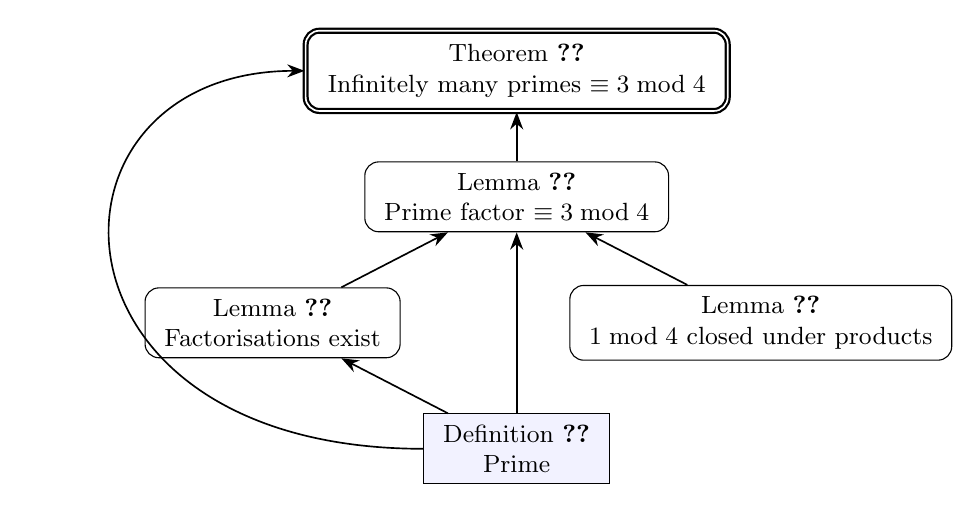
\begin{tikzpicture}[
  font=\small,
  defn/.style={draw, rectangle, align=center, inner xsep=7pt, inner ysep=4pt, fill=blue!5},
  lem/.style={draw, rounded corners=5pt, align=center, inner xsep=7pt, inner ysep=4pt},
  thm/.style={draw, double, rounded corners=5pt, align=center, inner xsep=8pt, inner ysep=5pt, thick},
  dep/.style={-{Stealth[length=2.2mm]}, semithick}
]
\node[thm]  (T6) at (0,0)       {Theorem~\ref*{ex:T6}\\ Infinitely many primes $\equiv 3 \bmod 4$};
\node[lem]  (L5) at (0,-1.6)    {Lemma~\ref*{ex:L5}\\ Prime factor $\equiv 3 \bmod 4$};
\node[lem]  (L2) at (-3.1,-3.2) {Lemma~\ref*{ex:L2}\\ Factorisations exist};
\node[lem]  (L3) at (3.1,-3.2)  {Lemma~\ref*{ex:L3}\\ $1 \bmod 4$ closed under products};
\node[defn] (D1) at (0,-4.8)    {Definition~\ref*{ex:D1}\\ Prime};
\draw[dep] (D1) -- (L2);
\draw[dep] (D1) -- (L5);
\draw[dep] (L2) -- (L5);
\draw[dep] (L3) -- (L5);
\draw[dep] (L5) -- (T6);
\draw[dep] (D1.west) .. controls (-6.2,-4.8) and (-6.2,0) .. (T6.west);
\end{tikzpicture}
\end{center}

\begin{hffdef}[Prime]\label{ex:D1}
An integer $p > 1$ is \emph{prime} if its only positive divisors are $1$ and $p$.
\end{hffdef}

\begin{hfflem}[Factorisations exist]\label{ex:L2}
Every integer $n > 1$ is a product of primes.
\end{hfflem}
\begin{proof}\setcost{length 159/300}
We use strong induction on $n$. If $n$ is prime, we are done. Otherwise, by \cref{ex:D1}, $n = ab$ for some integers $1 < a, b < n$. By the induction hypothesis $a$ and $b$ are products of primes, and hence so is $n$.
\end{proof}

\begin{hfflem}[$1 \bmod 4$ closed under products]\label{ex:L3}
If $a \equiv b \equiv 1 \pmod 4$, then $ab \equiv 1 \pmod 4$.
\end{hfflem}
\begin{proof}\setcost{length 69/300}
Write $a = 4s + 1$ and $b = 4t + 1$ with $s, t$ integers. Then
\[
  ab = 16st + 4s + 4t + 1 = 4(4st + s + t) + 1. \qedhere
\]
\end{proof}

\begin{hffrem}[What comes next]\label{ex:R4}
\Cref{ex:L2,ex:L3} are routine. The next lemma is the heart of the argument: it combines them to show that the residue $3$ cannot be built out of primes that are all $\equiv 1 \pmod 4$.
\end{hffrem}

\begin{hfflem}[Prime factor $\equiv 3 \bmod 4$]\label{ex:L5}
If $n > 1$ and $n \equiv 3 \pmod 4$, then some prime $p \equiv 3 \pmod 4$ divides $n$.
\end{hfflem}
\begin{proof}\setcost{length 151/300}
By \cref{ex:L2}, $n = p_1 \cdots p_r$ with each $p_i$ prime. Since $n$ is odd, each $p_i$ is odd, so $p_i \equiv 1$ or $3 \pmod 4$. If every $p_i \equiv 1 \pmod 4$, then $n \equiv 1 \pmod 4$ by \cref{ex:L3} applied $r - 1$ times, which is a contradiction.
\end{proof}

\begin{hffthm}[Infinitely many primes $\equiv 3 \bmod 4$]\label{ex:T6}
There are infinitely many primes $p \equiv 3 \pmod 4$.
\end{hffthm}
\begin{proof}\setcost{length 174/300}
The prime $3$ is one. Suppose $p_1, \dots, p_k$ are all of them, and let $N = 4p_1 \cdots p_k - 1$. Then $N > 1$ and $N \equiv 3 \pmod 4$, so by \cref{ex:L5} some prime $p \equiv 3 \pmod 4$ divides $N$. Then $p = p_i$ for some $i$, so $p$ divides $4p_1 \cdots p_k - N = 1$, which is absurd.
\end{proof}

\begin{hffrem}[Why subtract one]\label{ex:R7}
The $-1$ is what makes $N \equiv 3 \pmod 4$. Taking $N = 4p_1 \cdots p_k + 1$ instead gives $N \equiv 1 \pmod 4$, and \cref{ex:L5} says nothing about such numbers.
\end{hffrem}

\begin{hffrem}[The residue $1$]\label{ex:R8}
There are also infinitely many primes $\equiv 1 \pmod 4$, by Dirichlet's theorem on primes in arithmetic progressions~[Dir], but this argument does not show it. The analogue of \cref{ex:L3} for the residue $3$ fails, since $3 \cdot 3 \equiv 1 \pmod 4$, and so a number $\equiv 1 \pmod 4$ need not have a prime factor $\equiv 1 \pmod 4$; for example, $21 = 3 \cdot 7$.
\end{hffrem}

\medskip
\noindent\textbf{References}

\smallskip
{\small
\begin{enumerate}[leftmargin=3.2em, itemsep=2pt]
  \item[{[Dir]}] P.~G.~L. Dirichlet, \emph{Beweis des Satzes, dass jede unbegrenzte arithmetische Progression, deren erstes Glied und Differenz ganze Zahlen ohne gemeinschaftlichen Factor sind, unendlich viele Primzahlen enth\"alt}, Abh. K\"onigl. Preuss. Akad. Wiss. Berlin (1837), 45--81.
  \item[{[Euc]}] Euclid, \emph{Elements}, Book IX, Proposition 20.
\end{enumerate}
}
\end{tcolorbox}

A reader following \cref{proc:check} would read the overview and travel to \cref{ex:T6} on the map; confirm that it states the intended theorem and that \cref{ex:D1} is the usual notion of prime; note that there are no imported lemmas, since the references are cited only in the overview and a remark; and then check \cref{ex:T6}, \cref{ex:L5}, \cref{ex:L2} and \cref{ex:L3} in that order, each a single short proof. With the definition already confirmed, the map is then clear of fog and the theorem is proved.

% ==================================================================
\section{Open questions}\label{sec:open}
% ==================================================================

\begin{enumerate}[leftmargin=2em, label=(\arabic*)]
  \item \textbf{Calibration.} What value of $L$ makes checking fastest and most reliable, and how does it depend on the field?
  \item \textbf{Scale.} For a proof with thousands of lemmas, the map needs more structure, for instance modules that appear as named regions when zoomed out and open into their lemmas when zoomed in. Which layouts stay readable at that scale and stable under refinement?
  \item \textbf{Good decompositions.} \ref{H:short} can be met by chopping a proof into many lemmas with no natural content (\cref{rem:gaming}). Is there a useful measure of the quality of a decomposition?
  \item \textbf{Evidence.} Do readers in fact find errors faster and more reliably in \HFF{} than in a conventional write-up? One test is to plant errors in AI-generated proofs and compare how often they are caught in each form.
\end{enumerate}

\section*{Acknowledgements}

The core idea of this note is the author's: asking an AI to present its proof in the Human Friendly Form, checking that proof one short lemma at a time, and finding one's way through it on an interactive map of its dependency graph. Claude, an AI model developed by Anthropic, was responsible for the write-up under the author's direction. It put the author's ideas into clear English, typeset the note in \LaTeX, drew the figures, and built the worked example and the prototype map. The rule in \cref{sec:formulas} for measuring the length of a proof, by counting the visible characters of the compiled document with no exemption for formulas, is the author's; it replaces a rule proposed by Claude in an earlier version of this note, which treated formulas separately. Some other details were proposed by Claude and adopted by the author, such as conditions \ref{H:order}--\ref{H:inert}.

\begin{thebibliography}{9}

\bibitem{Leiden}
J.~Alper, M.~Barany, A.~Chavarri Villarello, S.~Dahmen, W.~Dean, K.~Ganapathy, M.~Harris, D.~Holmes, M.~Jamnik, S.~Kelk, B.~Kra, U.~Martin, B.~Naskr\eogonek cki, R.~Ochigame, J.~Portegies and J.~Schmitt, \emph{Leiden Declaration on Artificial Intelligence and Mathematics}, Zenodo, 2~June 2026, \href{https://doi.org/10.5281/zenodo.20302944}{doi:10.5281/zenodo.20302944}. Available at \url{https://leidendeclaration.ai/}.

\bibitem{AoE}
Ensemble Studios, \emph{Age of Empires}, video game, Microsoft, 1997.

\bibitem{Lamport1995}
L.~Lamport, \emph{How to write a proof}, Amer. Math. Monthly \textbf{102} (1995), no.~7, 600--608.

\bibitem{Lamport2012}
L.~Lamport, \emph{How to write a 21st century proof}, J. Fixed Point Theory Appl. \textbf{11} (2012), 43--63.

\bibitem{Tao}
T.~Tao, \emph{Mathematics in the age of AI}, preprint, 2026, \href{https://arxiv.org/abs/2608.16753}{arXiv:2608.16753} [math.HO].

\end{thebibliography}

\end{document}
